% Chapter 1
\chapter{Theory} % Main chapter title

\label{Chapter2} % For referencing the chapter elsewhere, use \ref{Chapter1} 

\lhead{Chapter 2. \emph{Theory}} % This is for the header on each page - perhaps a shortened title

%----------------------------------------------------------------------------------------

%----------------------------------------------------------------------------------------

\section{Mathematical Description}
In our study of CT-scan, we will consider a 2D slice of the
sample and assume which lies and centered on the XY-plane.

%\begin{figure}
%\begin{center}
%   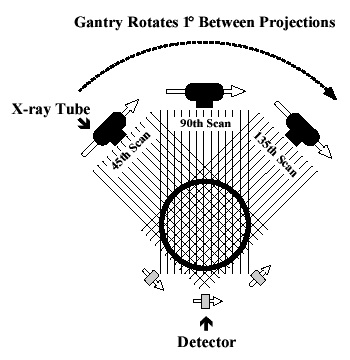
\includegraphics[width=210pt]{Figures/g1CT.jpg}
%   \caption{CT Scanner using parallel beam geometry}
%  \label{CTmodel}
%\end{center}
%\end{figure}

\begin{figure}[htbp]
	\centering
		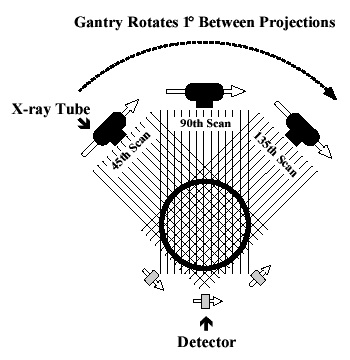
\includegraphics[width=210pt]{Figures/g1CT.jpg}
	\caption[CT scanner model]{CT Scanner using parallel beam geometry.}
	\label{fig:CTmodel}
\end{figure}


The relationship between measured intensity data ($I_0 $ :Intensity at source end, $ I_1 $ :Intensity at detector end) and attenuation-coefficients $f(x,y)$ of the material can be found by the Beer's law \cite{TimothyBook}. That is given by
\begin{equation}
ln \left( \frac{I_0}{I_1}\right) = \int_{x_0}^{x_1} f(x,y) ds.
\end{equation}
Once we parametrize the above integral along some line $l_{t,\theta}$ is called the \textit{Radon transform} and which is given by
\begin{equation}
\mathscr{R} f(t,\theta):= \int_{l_{t,\theta}} f ds=\int_{s=-\infty}^{\infty} f(tcos(\theta)-ssin(\theta),tsin(\theta)+scos(\theta))ds.
\end{equation}
Now our fundamental question is to find the function $f(x,y)$ if we know the total accumulation of the attenuation-coefficient function $f$ along every line that passes through the region. Suppose if we select some point in the plane, call it $(x_0,y_0)$, then which lies on many different lines in the plane. The first step in recovering $f(x_0, y_0)$ is to compute the average value of these line integrals averaged over all lines that pass through $(x_0, y_0)$.  This integral provides the motivation for the \textit{back-projection transform}. The back-projection of the Radon transform at $(x_0, y_0)$ is given by 

\begin{equation}\label{backproj}
\mathscr{B}\mathscr{R}f(x_0,y_0):=\dfrac{1}{\pi} \int_{\theta=0}^{\pi}\mathscr{R}f(x_0\cos(\theta)+y_0\sin(\theta),\theta) d\theta
\end{equation}
Hence, the value of the Radon transform along a given line would be the same if all of the matter there were replaced with a homogeneous sample whose attenuation coefficient was the average of the actual sample. Then the integral in equation (\ref{backproj}) is computing the average value of those averages. Thus, we can see this back-projection does not necessarily produce the exact value of $f(x_0,y_0)$. Instead it gives us an "smoothed-out" version of the attenuation coefficient.
In order to solve this problem, it is good to know the interaction between the Fourier transform and the Radon transform that is known as \textit{central slice theorem}.
\paragraph{Theorem 2.1. Central slice theorem.} For any suitable $f$ defined in the plane and all real numbers $S$ and $\theta$,
\begin{equation}\label{slice}
\mathscr{F}_2 f(S \cos(\theta), S \sin(\theta)) = \mathscr{F} (\mathscr{R} f) (S,\theta)
\end{equation}
The theorem (2.1), can be used derive new formula called the "\textit{filtered back-projection formula}" to correct the smoothing effect and recover the original function $f$.

For any suitable function $f$ and any point $(x,y)$ in the plane, by Fourier inversion theorem we can get
$$
f(x,y)=\mathscr{F}^{-1}_{2} \mathscr{F}_{2} f(x,y).
$$
By applying the definition of 2D inverse Fourier transform,
\begin{equation}\label{eq1}
f(x,y)=\dfrac{1}{4 \pi^2} \int^{\infty}_{-\infty} \int^{\infty}_{-\infty} \mathscr{F}_{2}f(X,Y) e^{i (xX+yY)} dX dY.
\end{equation}
Now change the variables such that $X=S \cos(\theta)$ and $Y=S \sin(\theta)$ where $0 \leq \theta \leq \pi \text{ and } S \in \mathbb{R}$. 
With these changes, equation (\ref{eq1}) becomes,
\begin{equation}\label{eq2}
f(x,y)=\dfrac{1}{4 \pi^2} \int^{\pi}_{0} \int^{\infty}_{-\infty} \mathscr{F}_{2}f(S\cos(\theta),S\sin(\theta)) e^{i S (x\cos(\theta)+y\sin(\theta))} |S|dS d\theta.
\end{equation}
Now with use of the central slice theorem (\ref{slice}), we can derive the "\textit{filtered back-projection formula}",
\begin{equation}\label{fback}
f(x,y) = \dfrac{1}{2} \mathscr{B} \left\lbrace  \mathscr{F}^{-1}\left[ |S|\mathscr{F} (\mathscr{R}f)(S,\theta) \right]  \right\rbrace (x,y).
\end{equation}
The filtered back-projection formula (\ref{fback}) is the fundamental basis for image reconstruction. Without the factor of $|S|$ in the formula, the Fourier transform and its inverse would cancel out and the result would be simply the back projection of the Radon transform of $f$ (see equation \ref{backproj}), which we know does not lead to recovery of $f$. Thus, the essential component in the formula is the $|S|$. Therefore we say that the Fourier transform of $\mathscr{R}f$ is filtered by multiplication by $|S|$.\\

\noindent
In practice, the above recipe for reconstructing $f$ has a problem. If the  $\mathscr{R}f$ has a component at high frequency, then that component is magnified by the factor $|S|$. This leads to exaggerate the noise by the same factor $|S|$ and which corrupts the reconstructed image. Thus, in practice, we replace $|S|$ by low-pass filter $A$.  
Then after some algebraic simplifications, function $f$ can be approximated by
\begin{equation}\label{modeqn}
f(x,y) \approx \frac{1}{2} \mathscr{B}(\mathscr{F}^{-1}A \; * \; \mathscr{R}f)(x,y),
\end{equation}
where, $(*)$ denotes the convolution of $\mathscr{F}^{-1}A$ and $\mathscr{R}f$. \\

\noindent
Here are some of the low-pass filters most commonly used in medical imaging. 

\begin{itemize}
\item[1.] The Ram-Lak filter:
\begin{eqnarray} \nonumber
A_1(\omega) = |\omega| \cdot \sqcap_{L}(\omega) = \left\{
\begin{array}{ll}
 |\omega | &\text{if } |\omega | \leq L,\\
 & \\
0 & \text{if  } |\omega | > L.\\
\end{array} \right.
\end{eqnarray}

\item[2.] The Shepp-Logan filter:
\begin{eqnarray}
A_2(\omega) &=& |\omega | \cdot \left( \frac{\sin(\pi \omega / (2L))}{\pi \omega / (2L)}\right) \cdot \sqcap_{L}(\omega) \nonumber \\
 &=& \left\{
\begin{array}{ll}
 \dfrac{2L}{\pi} |\sin(\pi \omega / (2L))| & \text{if } |\omega | \leq L,\\
 & \\
0 & \text{if  } |\omega | > L.\\
\end{array} \right. \nonumber
\end{eqnarray}

\item[3.] The Low-pass Cosine filter:
\begin{eqnarray}
A_3(\omega) &=& |\omega | \cdot \cos(\pi \omega / (2L)) \cdot \sqcap_{L}(\omega) \nonumber \\
 &=& \left\{
\begin{array}{ll}
 |\omega |\cos(\pi \omega / (2L)) & \text{if } |\omega | \leq L,\\
 & \\
0 & \text{if  } |\omega | > L.\\
\end{array} \right. \nonumber
\end{eqnarray}
\end{itemize} 



\section{Discrete Mathematical Model}
In the discrete setting, let's implement the filtered back-projection formula (\ref{modeqn}) as
$$
f(x, y) \approx   \frac{1}{2} \mathscr{B}_D \left( \mathscr{I} \left( \mathscr{F}^{-1}_{D} A \; \bar{*} \; \mathscr{R}_D f \right)\right)(x, y),
$$
where each term is described below. 
\subsection{$\mathscr{R}_Df$ is the discrete Radon transform.}
Discrete Radon transform is given by
$$
\mathscr{R}_D f_{j,k} = \mathscr{R}f (jd,k\pi/N),
$$
for $-M \leq j \leq M$ and $0 \leq k \leq (N-1)$. Suppose that there are $2\cdot M + 1$ parallel X-ray beams at each angle, $N$ different scans and beam spacing is $d$ .\\
\begin{figure}[H]
	\centering
		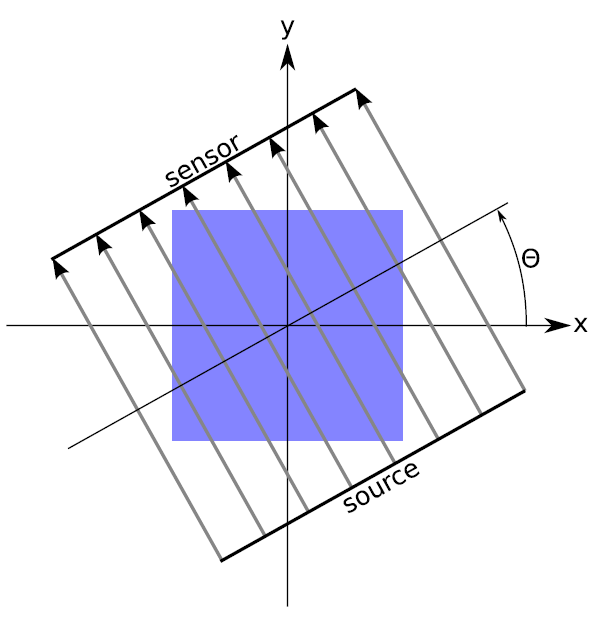
\includegraphics[width=230pt]{Figures/radon.png}
	\caption[Radon transform]{The Radon transform is a mapping from the Cartesian rectangular coordinates $(x,y)$ to a distance and an angel $(t, \theta)$, also known as polar coordinates.}
	\label{fig:radon}
\end{figure}

Finding $\mathscr{R}_D f_{j,k}$ can be thought of as computing the projection of the image along the $k$th angle and $j$th beam. The resulting projection is the sum of the intensities of the pixels along that line, i.e. a line integral. This is depicted in Figure \ref{fig:radon} \cite{Radon}.  

In order to reduce the number of calculations necessary, the maximum and minimum coordinates x or y are determined for each line (for more details see Appendix \ref{AppendixA}). 

\begin{figure}[H]
	\centering
		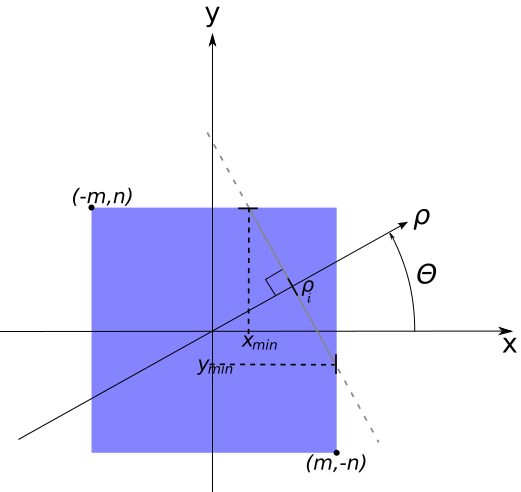
\includegraphics[width=230pt]{Figures/minmax.png}
	\caption[Maximum and minimum coordinates of x or y.]{Determining the maximum and minimum coordinates.}
	\label{fig:minmax}
\end{figure}


\subsection{$\mathscr{F}^{-1}_{D} $ is the discrete inverse Fourier transform.}
Samples for $\mathscr{F}^{-1}_{D} $ can be generated for the Shepp-Logan, Ram-Lak and low-pass cosine filters using Nyquist distance $\pi/L$ \cite{charles}.\\
Samples for discrete inverse Fourier transform of Shepp-Logan filter$(A)$ is given by
$$
(\mathscr{F}^{-1}_{D} A)_n =  \frac{4L^2}{\pi^3 (1-4n^2)}
$$
Samples for discrete inverse Fourier transform of Ram-Lak filter$(A)$ is given by
\begin{eqnarray}
\left(\mathscr{F}^{-1}A\right)_n &=& \frac{L^2}{2\pi}\left[ \frac{2\sin(\pi n)}{\pi n}-\left(\frac{\sin(\frac{\pi n}{2})}{\frac{\pi n}{2}}\right)^2 \right].\nonumber
\end{eqnarray}
If $n=0$: $(\mathscr{F}^{-1}A)(0) = L^2/2\pi$ \\
If $n$ is even : $(\mathscr{F}^{-1}A)(\frac{\pi n}{L})=0$ \\
If $n$ is odd : $(\mathscr{F}^{-1}A)(\frac{\pi n}{L})= -2L^2/(\pi^3 n^2)$\\
Samples for discrete inverse Fourier transform of low-pass cosine filter$(A)$ is given by
\begin{eqnarray}
\left(\mathscr{F}^{-1}A\right)\left(\frac{\pi n}{L}\right)&=&
\frac{2L^2}{\pi^3} \Big\lbrace  \frac{\pi \cos(\pi n)}{(1-4n^2)} -  \frac{2(4n^2+1)}{(1-4n^2)^2} \Big\rbrace \nonumber
\end{eqnarray}
The band limit $L$ in each above formulas can be found by 
$$
L = \frac{1}{2d},  \qquad \text{where } d \text{ is the beam spacing. }
$$
Fast Fourier transform also can be used to obtain the samples for each filter. 

\subsection{($\bar{*}$) denotes the discrete convolution.}
For two $N$-periodic discrete functions $g$ and $h$, the discrete convolution is defined by
$$
(g \ \bar{*} \ h)_m = \sum_{j=0}^{N-1} g_j \cdot h_{(m-j)} \text{ for each integer } m.
$$ 
\subsection{$\mathscr{I}$ is the $W$-interpolation function.}
It is defined for some discrete function $g$ as
$$
\mathscr{I}_W(g)(x) = \sum_m g(m) \cdot W\left( \frac{x}{d}-m \right) \qquad \text{for } -\infty < x < \infty. 
$$
If $W$ weighting function is square wave function,\\
i.e.
\begin{eqnarray}
\sqcap_{1/2}(x) &=& \left\{
\begin{array}{ll}
1 & \text{if } |x| < 1/2,\\
 & \\
0 & \text{if } |x| > 1/2 .\\
\end{array} \right. \nonumber
\end{eqnarray}
then it is called \textit{nearest neighbor} interpolation.\\
If $W$ is tent function,\\
i.e.
\begin{eqnarray}
\bigwedge(x) &=& \left\{
\begin{array}{ll}
1 & \text{if } |x| \leq 1,\\
 & \\
0 & \text{if } |x| > 1 .\\
\end{array} \right. \nonumber
\end{eqnarray}
then it is called \textit{linear} interpolation.  

\subsection{$\mathscr{B}_D$ is the discrete back projection.} 
For some function $h$, discrete back projection is given by
$$
\mathscr{B}_D h(x,y) = \left(\frac{1}{N}\right) \sum_{k=0}^{N-1} h(x \cos(k \pi/N)+ y \sin(k \pi/N), k \pi/N).
$$
\section{Discrete Image Reconstruction Algorithm}
By combining the all above discrete models together, we can derive the discrete image reconstruction algorithm in abstract manner \cite{TimothyBook}.\\
In the reconstruction grid, we approximate the gray scale intensity at each lattice point $(x_m, y_n)$ by
\begin{eqnarray}\label{algo}
f(x_m, y_n) &\approx & \left( \frac{1}{2}\right) \mathscr{B}_D \left( \underbrace{\mathscr{I} \left( \mathscr{F}^{-1}_{D} A \; \bar{*} \; \mathscr{R}_D f \right)}_{\mathscr{I}_0}(t,k\pi /N) \right) (x_m, y_n)  \\
&=& \left( \frac{1}{2N}\right) \sum_{k=0}^{N-1} \mathscr{I}_0  \left(x_m \cos \left(\frac{k \pi}{N}\right) + y_n \sin\left(\frac{k \pi}{N}\right), \frac{k \pi}{N}\right).\nonumber
\end{eqnarray}